\documentclass[kp]{foilpack}
%\documentclass{mediumfoils}
 
\usepackage{ctable}
\usepackage{fancyvrb}

\graphicspath{{/Users/will/Dropbox/pictures/}{/Users/will/Dropbox/}} 
%% add an extra path if you've moved the X in X/pictures/ someplace



\talktitle{3. Positions}
\author{\textbf{Will Lowe}\\University of Mannheim \and
 \textbf{Sven-Oliver Proksch}\\McGill University}

\date{}
\runningfooter{IQMR, June 2014}

\begin{document}

\maketitle

\slide{Menu}

Session 1: Classical Content Analysis

Session 2: Topic Models and Classification

Session 3: 
\ita
\itm Scaling Models
\ita
\itm How to take a position using words: pre-coded data
\itm Scaling models
\itm Dimensionality
\itm Scaling in institutional context
\itz
\itz

\slide{Assume the Position}

Some Politics:
\ita
\itm Actors \textit{generate}, \textit{infer}, \textit{change} and \textit{frame} positions on continuous policy dimensions
\itz

Some Methods:
\ita
\itm Scaling models explain the generation and the inference parts
\itm \textit{Vote} scaling models explain how they do it with votes; \textit{text} scaling models explain how they do it with text
\itz

\slide{Intuition}

\textbf{positions are \textit{low dimensional reconstructions} of \textit{patterns of relative emphasis}}

(Generalising the simple difference measures we constructed before from categories)

%\slide{Positions from Political Texts}   
%	
%\ita
% \itm  Our measurement approach should be ideally motivated by theory     
% \itm  Some types of political behavior are more likely to be of strategic nature than others 
% 
%   \itm You should be aware of the context when analyzing political texts 
%	\ita
%   \itm --  Campaign platforms (election manifestos)
%   \itm -- Parliamentary Speeches
%   	\itz
%
%\itz
%
%
%
%\slide{Positions from Political Texts}   
%
%Think about the data-generating mechanism of your data.
%   
%  
%
% \begin{enumerate}
%
% \item In what context do political actors express an opinion? 
% \item Are there constraints on the language used? 
% \item Do the same context and the same constraints apply to all documents in your corpus?
% \item Consider the implications for the choice of measurement approach
% 
%
%   \end{enumerate}
%





\slide{The Manifesto Research Project}

Manifesto Research Project (has been going on under various labels since 1979: MRG, CMP, MARPOR)

 Text collection: party  manifestos since 1945 

	 584 elections, 3334 manifestos, 55 countries,	840 parties 
	 
 By far the largest content analysis endeavor in political science 
	
One of  most frequently used datasets in comparative politics: three major  publications with over 1,000 Google scholar citations



\slide{How to Measure Position: The Manifestos Project}

Code each argument (so-called quasi-sentence) into one of 56 policy categories + uncodable

 This is essentially (extremely complex) classification (and unitization)

 Codings are percentage of "quasi-sentences" falling into these categories	 


\slide{Of Luddites and Masochists}

I don't trust these crazy models and their unlikely assumptions.  I'm going to do it all myself\footnote{By `myself' I mean my graduate students, postdocs and interns}.

Classic example: The CMP (Budge et al. 1992)

For each post war party manifesto (or closest document)
\ita
\itm Identify distinct policy assertions `quasi-sentences'
\itm Categorize each sentence in one of 56 categories, according to the codebook
\itm Construct left-right measures by \textit{subtracting opposing category proportions}
\itz

\slide{Newsflash}

Manual coding is hard

\slide{Newsflash}

Hard = not necessarily \textit{valid} and not necessarily \textit{reliable}

\ita
\itm Valid: I put things in the right categories
\itm Reliability: I would categorize the same way again tomorrow \textit{or} My colleague would categorize the same way as me today
\itz

%\slide{Types of Validity}
%
%\begin{center}\includegraphics[scale=.15]{pictures/validity-typology}\end{center}
%
%\slide{Validity and Reliability}
%
%\begin{center}\includegraphics[scale=.15]{pictures/targets}\end{center}
%
%\slide{Validity and Reliability}
%
%\begin{center}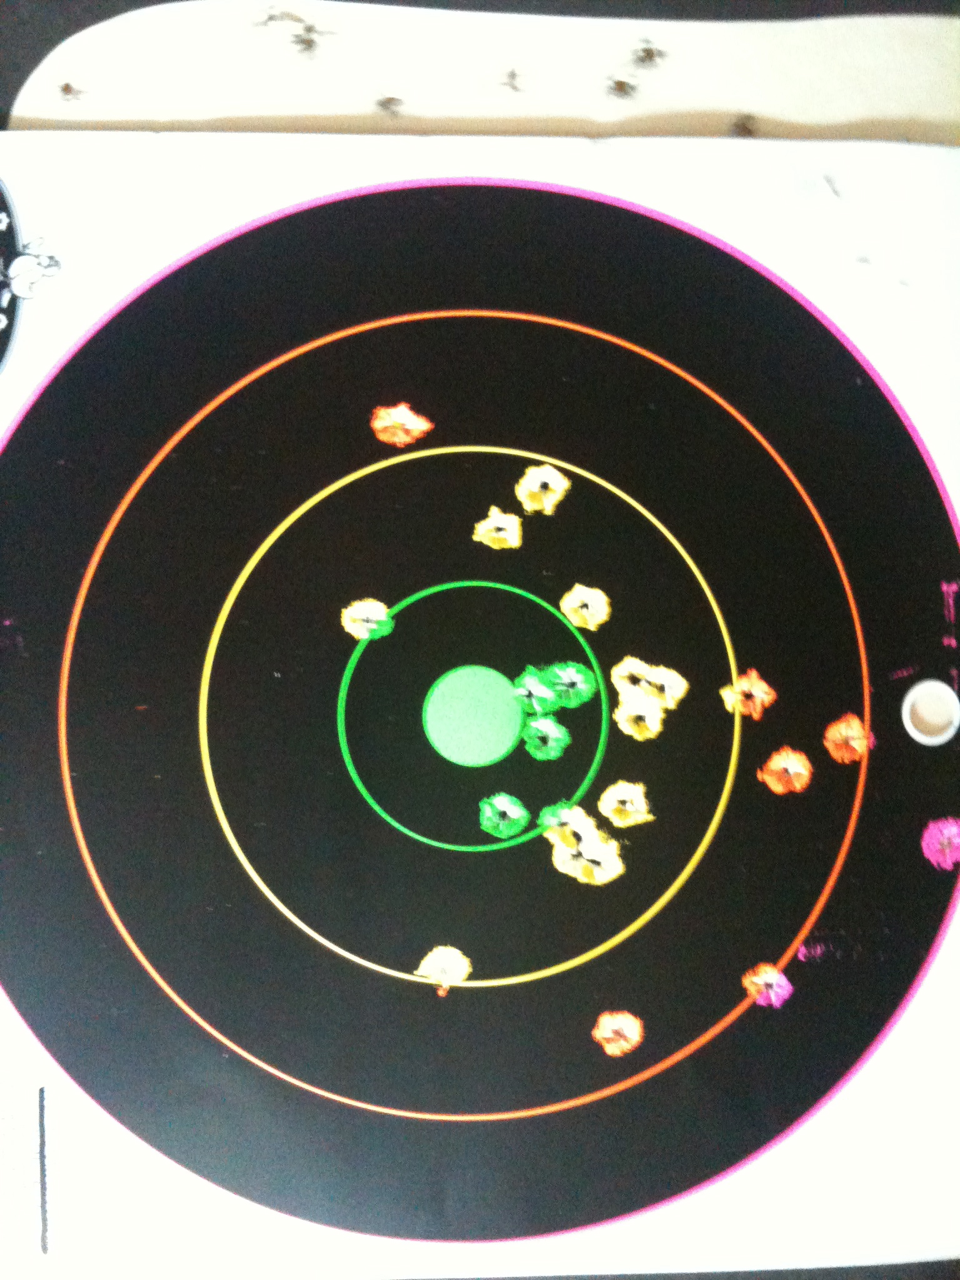
\includegraphics[scale=.2,angle=270]{pictures/wl-targets3}
%~~~~~~~~~~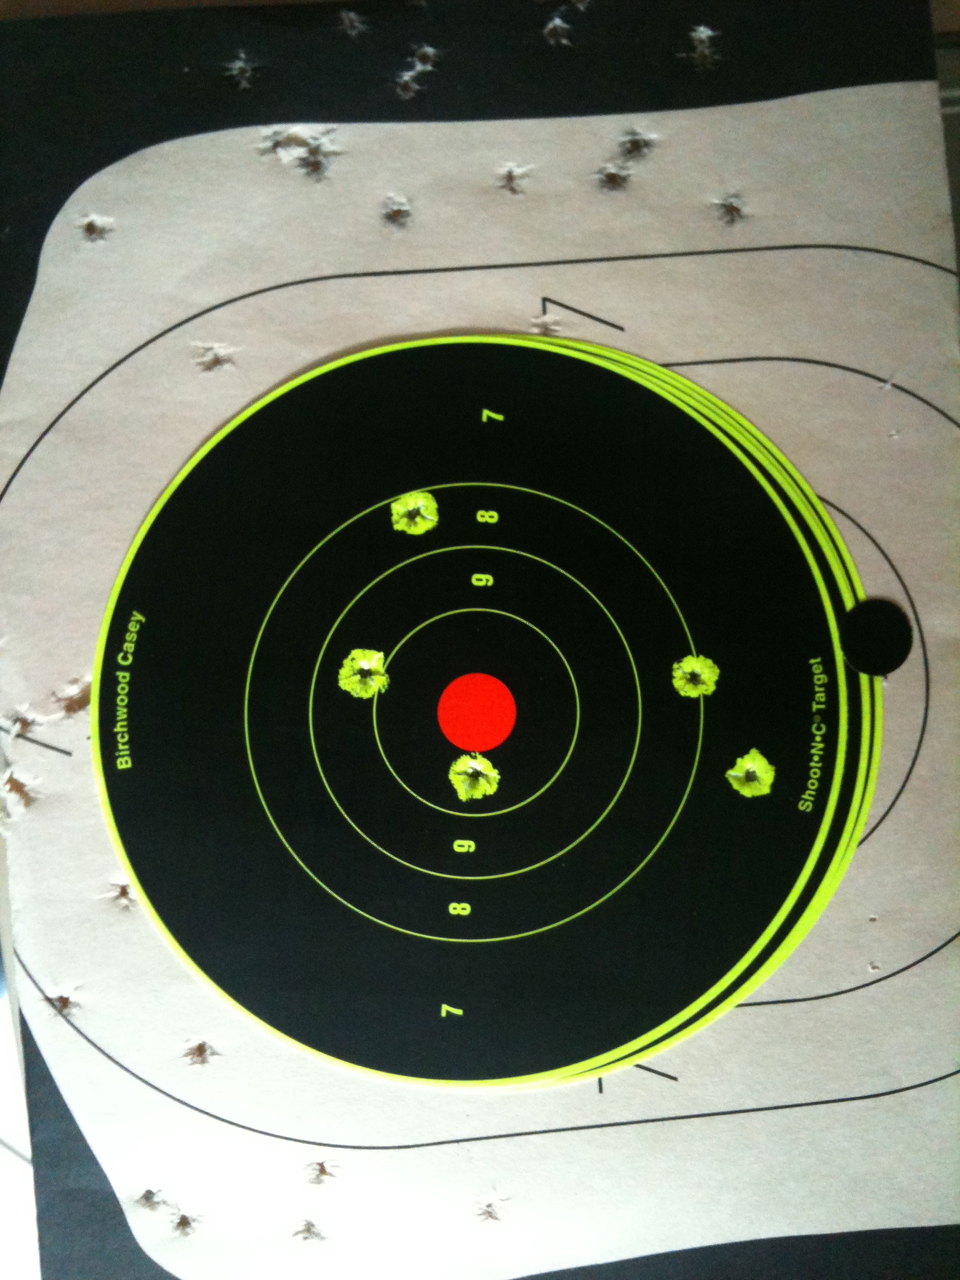
\includegraphics[scale=.2,angle=270]{pictures/wl-targets4}\end{center}
%


\slide{How bad could we be?}

\begin{center}\includegraphics[scale=.7]{pictures/reltestRILE}\end{center}

\slide{How bad could we be?}

\begin{center}\includegraphics[scale=.9]{pictures/nQSreltest}\end{center}

\slide{Measurement Error and its effects}

Notice that this problem arises for machine and manual coding -- \textit{both} may make a coding mistake

\begin{center}
\includegraphics[scale=.4]{pictures/comparison}
\end{center}

\slide{Mechanical Turk}

\centerline{\includegraphics[scale=.4]{turk}}

\slide{Mechanical Turkers}

\centerline{\includegraphics[scale=.5]{mturkers}}

\slide{Mechanical Turkey}

\centerline{\includegraphics[scale=.6]{mturking}}

\slide{Mechanical Turkish Delight}

\centerline{\includegraphics[scale=.8]{mturk2}}


\slide{}

\slide{Positions from Pre-Coded Sentences}

Now W is counts of manually pre-coded sentences

~\\
\centerline{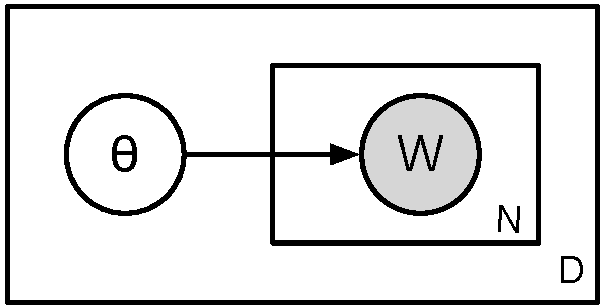
\includegraphics[scale=.9]{scalingmodels}} 

%~~~~~~~~~~versus~~~~~~~ \includegraphics[scale=.7]{topics-ca}}

~\\
But now new \textit{choices about the mapping}.  What is $\theta$ $\longrightarrow$ W?


\slide{$\theta \longrightarrow$ W (CMP-style)}

Raw materials
\ita
\itm N sentences in a party manifesto
\itm L sentences coded into categories on one side of the issue
\itm R sentences coded into categories on the other side of the issue
\itz

~\\
How does $\theta$ relate to R and L in a document N words long?
\ita
\itm Let us count (some) ways\ldots
\itz

\slide{How To Measure Position: The Manifestos Project}

Intuition: The \textsl{difference} between right and left.

Comparative Manifesto Project position (from saliency theory)
\[
\theta^{(S)} ~=~ \frac{R-L}{N}
\]
Marginal effect: 1/N

Problems:
\ita
\item[-] Fixed (but hidden) end points
\item[-] Position depends on attention to \textit{other} issues  
\itz

\slide{How To Measure Position:\\Kim and Fording}

Intuition: The \textit{difference} between right and left \textsl{on topic}

Relative position:
\[
\theta^{(R)} ~=~ \frac{R-L}{R+L}
\]
Marginal effect: 1/(R+L)

Problem:
\ita
\itm Fixed end points (that are often reached)
\itz

(Kim and Fording 2002, Laver and Garry 2000)

\slide{How to Measure Position}

Intuition: The \textsl{balance} or \textit{relative emphasis} of R versus L

Empirical logit:
\[
\theta^{(L)} ~=~ \log\frac{R}{L} ~=~ \log(R) - \log(L)
\]

\textsl{No} fixed end points

Marginal effect: Depends on how much R or L there is already!

(Lowe et al. 2011)

\slide{How to Read a Text:\\ Marginal Effects}

A party manifesto from the most recent EP elections

\newpage

\footnotesize
Immigration is out of control.
\normalsize

\newpage

\footnotesize
Immigration is out of control.
\textbf{Britain's population is now over 60 million and rising, solely due to immigration.}
\normalsize

\newpage

\footnotesize
Immigration is out of control.
Britain's population is now over 60 million and rising, solely due to immigration.
\textbf{Not only is Britain increasingly overcrowded but the fact is that a country is the product of its people  and
if you change the people you will inevitably change the nature of the country.}
\normalsize

\newpage

\footnotesize
Immigration is out of control.
Britain's population is now over 60 million and rising, solely due to immigration.
Not only is Britain increasingly overcrowded but the fact is that a country is the product of its people  and
if you change the people you will inevitably change the nature of the country.
\textbf{We want Britain to remain - or return to - the way it has traditionally been.}
\normalsize

\newpage

\footnotesize
Immigration is out of control.
Britain's population is now over 60 million and rising, solely due to immigration.
Not only is Britain increasingly overcrowded but the fact is that a country is the product of its people  and
if you change the people you will inevitably change the nature of the country.
We want Britain to remain - or return to - the way it has traditionally been.
\textbf{We accept that Britain will always have ethnic minorities and 
have no problem with this as long as they remain minorities and
neither change nor seek to change the fundamental culture and identity of the indigenous peoples of the British Isles.}
\normalsize

\newpage

\footnotesize
Immigration is out of control.
Britain's population is now over 60 million and rising, solely due to immigration.
Not only is Britain increasingly overcrowded but the fact is that a country is the product of its people  and
if you change the people you will inevitably change the nature of the country.
We want Britain to remain - or return to - the way it has traditionally been.
We accept that Britain will always have ethnic minorities and 
have no problem with this as long as they remain minorities and
neither change nor seek to change the fundamental culture and identity of the indigenous peoples of the British Isles.\\
~\\
\textbf{The current open-door policy and unrestricted uncontrolled immigration is leading to higher crime rates, demand for more housing (driving prices out of the reach of young people), severe strain on the environment, traffic congestion, longer hospital waiting list, lower educational standards, higher income taxes, lower wages, higher unemployment, loss of British identity, a breakdown in community spirit, more restrictive policing, higher council tax rates, a shortage of council homes, higher levels of stress and unhappiness and a more atomized society.}
\normalsize

\slide{Functional Form?}

~\\
\centerline{\includegraphics[scale=1]{lambdaRinv}}

\slide{Functional Form}

~\\
\centerline{\includegraphics[scale=1]{lambdaR}}


\slide{The Psychophysics of\\ Left and Right}

Inferences about position operate like perceptions of loudness or perceived weight 

The smallest perceivable \textsl{policy position} difference (JND) depends on the extremity of the existing policy.

\ita
\itm This is the Weber-Fechner Law (Fechner, 1965)
\itz

\slide{The Psychophysics of\\ Left and Right}

~\\
Compare these possible measures to expert survey scores (Benoit and Laver, 2006)

\newpage

\begin{center}
    \includegraphics[scale=0.8]{pictures/proofSocial.pdf}
\end{center}
\newpage

\begin{center}
   \includegraphics[scale=0.8]{pictures/proofMulticult.pdf}
\end{center}
\newpage

\begin{center}
    \includegraphics[scale=0.8]{pictures/proofEnvt.pdf}
\end{center}

\slide{Just a Moment\ldots}

Did you say environmental policy positions?  Surely nobody says anything \textit{against} the environment

\slide{Just a Moment\ldots}

True.  They choose something else to emphasize instead\ldots

~\\
The Danish Liberal Party in 1988:

\ita
\itm ``Milj\o politikken m\aa ikke stille danske virksomheder d\aa rligere, end
  virksomhederne i de lande vi konkurrerer med''
\itm Environmental policy should not result in Danish companies
  being worse off than the companies in the countries with which we
  compete.
\itz

\slide{Other Possibilities}

\centerline{\includegraphics[scale=.6]{pictures/stevens.png}}

Stimulus intensity = more L (or R) words.\\
Sensation magnitude = position movement left (or right)

\slide{Not Yet a Model}

This is \textit{not} a  {model} of $\theta$, its dimensionality, determinants, or structure.  Just a way to figure out what it is from text.

This is a \textsl{noisy} scaling technique compared to, e.g. indexes from carefully focused survey questions or expert opinion.  A model will help here\ldots

The \textsl{form} of decreasing marginal effects -- here the log -- is assumed, and supported by comparison to expert scores

the logit (log both ways) is suitable when we have an `opposite side'

\slide{Statistical Models of Scaling}

How do we build this into a model?

~\\
\centerline{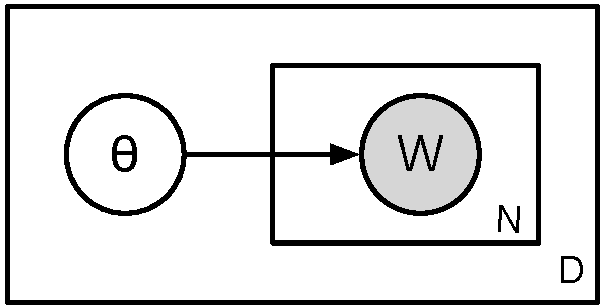
\includegraphics[scale=.9]{scalingmodels}}

Latent variable models, e.g.
\ita
\itm Factor Analysis, IRT / Latent Traits, Unfolding, Multidimensional Scaling, Wordfish,
Correspondence Analysis 
\itz


%\slide{Scaling Senate Output}

%\centerline{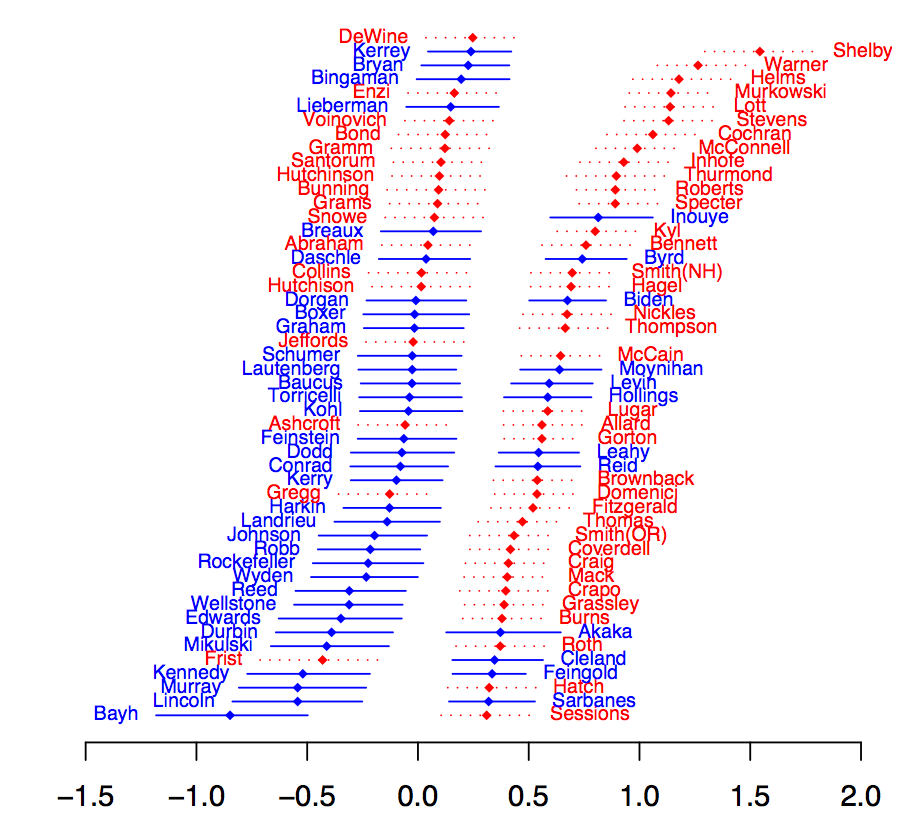
\includegraphics[scale=.45]{senator-ip-monroe-maeda}}



\slide{Assumptions}

Typically scaling models assume that
\ita
\itm relative word usage is reflective of political ideology
\itm Positions are unidimensional in $W$ 
\itm Positions drive word counts stochastically according to a particular form for $P(W_{j} \mid \theta)$
\itm Bag of words: counts of $W_{j}$ are conditionally independent given $\theta$
\[
P(W_{1}\ldots W_{V}) ~=~ \prod^{V}_{j} P(W_{j} \mid \theta)~ P(\theta)
\] 
\itz 

\slide{Existing Models}

We focus on:
\ita
\itm \textit{Wordfish}: (Slapin and Proksch, 2008)
\itm (Also Laver et al. 2003, Monroe and Maeda, 2004; Beauchamp, 2008; Pennings and Keman, 2002; K\"{o}nig and Luig, 2009, Goodman 1979, etc.)
\itz

%%%%%%%%%%%%%%%%%%%%%%%%%%%%%%%%%%%%%

\slide{Wordfish}

The position word relationship is
\begin{eqnarray*}
W_{ij} &\sim& \text{Poisson}(\mu_{ij})\\
\log \mu_{ij} &=& \psi_{j} + \beta_{j}\theta_{i} +  \alpha_{i} 
\end{eqnarray*}
Each word is a Poisson Process (stochastic component) driven by word and document parameters (the systematic component)


Word parameters:
\ita
\itm $\beta$~~ how fast counts increase or decrease with changes in position
\itm $\psi$~~ how frequent words are irrespective of position
\itz


\slide{Wordfish}

~\\
~\\
\centerline{\includegraphics[scale=.75]{log-lambda}\quad\quad\quad\includegraphics[scale=.75]{lambda}}

\slide{Wordfish}


Ideal data:
\footnotesize
\begin{verbatim}
    D1 D2 D3 D4 D5 D6 D7 D8 D9 D10
W1   6 12  5 13 30 19 38 43 44  47
W2   2  4  9  7 29 21 40 33 43  43
W3   6  3  2  6 20 27 28 42 47  49
W4   4  7  7  9 34 27 30 38 47  48
W5   2  6  7 13 25 36 24 31 32  52
...
W11 50 46 49 38 21 27 17  7  5   1
W12 53 39 46 35 20 26 18 10 12   4
W13 36 51 39 46 27 18 19  8  3   2
W14 46 46 43 43 24 20 13  7 10   1
W15 43 44 35 35 25 30 15  8 12   3
\end{verbatim}
\normalsize



\newpage


\centerline{\includegraphics[scale=.75]{sp-informativeness}}


\slide{Wordfish}

The position word relationship is
\begin{eqnarray*}
W_{ij} &\sim& \text{Poisson}(\mu_{ij})\\
\log \mu_{ij} &=& \psi_{j} + \beta_{j}\theta_{i} +  \alpha_{i}
\end{eqnarray*}
Each word is a Poisson Process driven by word and document parameters

Document parameters:
\ita
\itm $\theta$~~ the position being expressed
\itm $\alpha$~~ a fixed effects for documents controlling for length\ldots
\itz

%\slide{Wordfish}

%If document \textit{length} is uninformative about position then we can condition on it. 

%In fact Wordfish already does

%\begin{eqnarray*}
%P(W_{i} \mid \theta_{i}, N) &=& \text{Multinomial}(\boldsymbol{\pi}, N)\\
%\log \frac{\pi_{ij}}{\pi_{i1}} &=& \psi^{*}_{j} + \beta^{*}_{j}\theta_{i}
%\end{eqnarray*}
%where $\psi^{*}_{j} \leftarrow (\psi_{j}-\psi_{1})$, $\beta^{*}_{j} \leftarrow (\beta_{j}-\beta_{1})$ and $\alpha_{i}$ cancels

%~\\
%Wordfish is secretly a Multinomial Response Model

%\slide{Wordfish}
%
%This matters primarily for predicting the positions of new documents
%\ita
%\itm What $\alpha$ should a new document get?
%\itz
%Also for accurate standard errors
%\ita
%\itm Replace the parametric bootstrap procedure 
%\ita
%\itm ``it may take several days to estimate confidence intervals on a standard desktop computer'' (Wordfish FAQ)
%\itz
%\itm with a cheap asymptotic version
%\itz

\slide{Estimation}

Wordfish models are fit using Conditional Maximum Likelihood (regression without independent variables)
%\ita
%\itm (Not quite an EM algorithm)
%\itz

Iterate:
\ita
\itm Fix document parameters ($\alpha$ and $\theta$) and maximize word parameters ($\beta$ and $\psi$)
\itm Fix new word parameters ($\beta$ and $\psi$) and maximize document parameters ($\alpha$ and $\theta$)
\itz

This can be quite slow depending on the size of your dataset\ldots

%The model is slightly more stable when $\beta$ is regularized 
%\ita
%\itm Equivalent to assuming that $\beta \sim \text{Normal}(0,\sigma^{2})$ a priori
%\itz

%\slide{A Hint of Bayes}

%The iteration embeds an application of Bayes theorem:
%\ita
%\itm In step 2: Assume $P(\theta)$ is constant
%\begin{eqnarray*}
%P(\theta \mid W; \beta, \psi) &~\propto~& P(W \mid \theta; \beta, \psi)~ P(\theta)\\
%\text{Posterior} &~\propto~& \text{Likelihood} ~\times~ \text{Prior}\\
%\theta \Longleftarrow W & & W \longleftarrow \theta,\quad \theta
%\end{eqnarray*}
%Maximize this posterior distribution over $\theta$
%\itz
%~\\
%Note that the Likelihood is really $V$ Likelihoods, one for each word type\ldots


\slide{Wordfish: Model Identification}
\[\log \mu_{ij} = \psi_{j} + \beta_{j}\theta_{i} +  \alpha_{i}\]

	As is the case with all scaling models (e.g. NOMINATE), the likelihood function is not identified.
		
	  Without fixing some parameters, there are infinite combinations of $\theta$ and $\beta$, which could provide the same likelihood (we would not arrive at a unique solution). 
    

Solution: fix  mean of document positions %$\omega$ 
$\theta$ to 0 and St. Dev. to 1. Set one document fixed effect to 0. Set directionality of scale. This means that you cannot directly compare estimates ACROSS different estimations.


\slide{German Party Positions 1990-2005}

\centerline{\includegraphics[scale=.85]{poissonscaling}}


\slide{What about differences across languages?}




 Ideal case: get the exact same political texts in high quality translations

 Estimate Wordfish and compare across different languages

 This is possible: European Parliament speeches (translated into all official languages of the EU)




\slide{What about differences across languages?}

\begin{center}
Positions of National Parties in the European Parliament


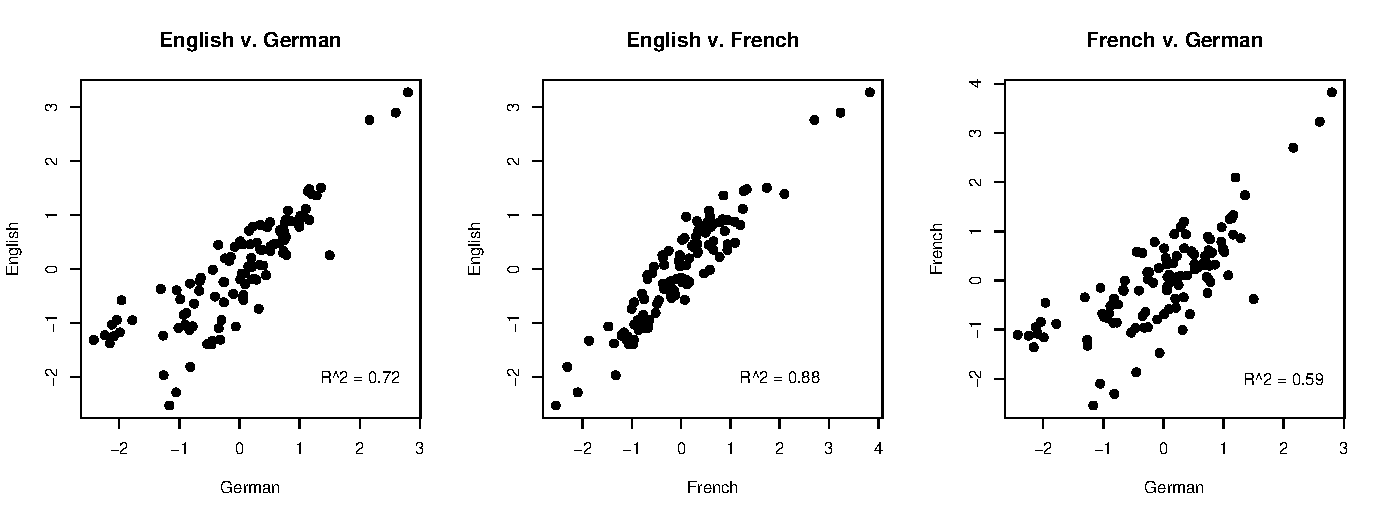
\includegraphics[width=24cm]{scatter_wordfish.pdf}

\end{center}



%\slide{Big Picture: As Measurement}
%
%\begin{center}
%\footnotesize
%\begin{tabular}{ccc}
%\textbf{Distance Measures} & \textbf{Dominance Measures} & \\
% &  & \\
%Parametric Unfolding & Item Response Theory & (Wordfish) \\ 
%$\uparrow$ & $\uparrow$ & \\
%\textsl{approx.} & \textsl{approx.} & \\
%$\mid$ & $\mid$ & \\
%Correspondence Analysis & Factor Analysis & \\
%$\uparrow$ & $\uparrow$ & \\
%\textsl{implements} & \textsl{approx.} & \\
%$\mid$ & $\mid$ & \\
%Reciprocal Averaging & PCA & \\
%$\uparrow$ & & \\
%\textsl{approx.} &  & \\
%$\mid$ & & \\
%Wordscores & & \\
%\end{tabular}
%\normalsize
%\end{center}
%



\slide{Dimension Issues}

What the heck is $\theta$?

How do we know that positions on only one dimension are being expressed in the text?

\slide{Dimension Issues}

What the heck is $\theta$?
\ita
\itm Whatever maximizes the Likelihood
\itm Approximately the first principal component of $\log W$ 
\itz
Like all scaling techniques (e.g. NOMINATE), Wordfish is effectively \textit{exploratory} -- you have to figure out what the dimension really is. This is the reason why you need to think about your data before applying the method.


\slide{Dimension Issues}

How do we know that positions on only one dimension are being expressed? How do we get positions on a specific policy issue?

\textit {Force} the assumption to be true by including substantive knowledge about your texts:
\ita
\itm Use only those texts (or sections thereof)  that are guaranteed to be on the same topic and scale them separately 

\itm E.g. speeches from a specific debate or policy sections of manifestos (e.g.  Slapin and Proksch 2008)
\itm Monroe and Quinn (endlessly forthcoming) use a topic model
\itz
Advantage: Heroic assumptions are (closer to being) true


\slide{Multiple Dimension Issues}

\centerline{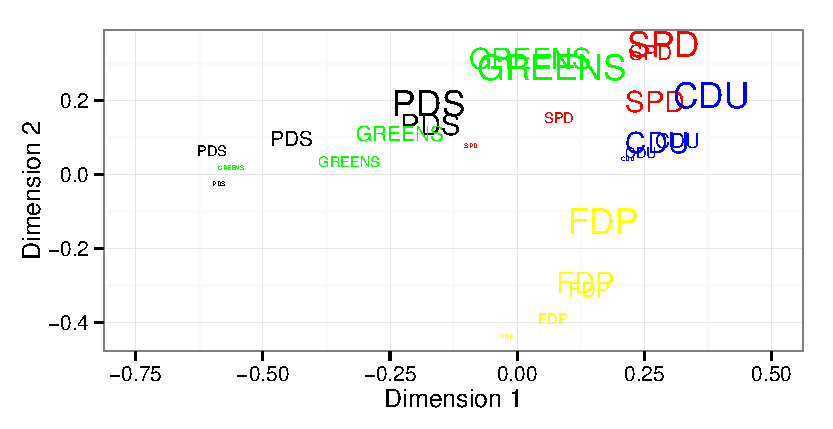
\includegraphics[scale=1]{de-2d}}


\slide{ (In)Stability of the Political Lexicon}

What if the political lexicon is unstable over time?
\ita
\itm New issues appear, old issues disappear
\itz


If this happens frequently, then scaling algorithms will pick up shifts in the policy agenda -- rather than shifts in party positions. 

\ita
\itm In fact, this is one assumption: that word usage reflects ideology.
\itm For example, it becomes seriously problematic when all parties start talking about the "issue" of the day. Then we can distinguish between elections, but not very well between parties
\itm We can (try to) get around this by focusing on those words that remain in the political vocabulary across time.
\itz


\slide{Worst Case Scenario}

\centerline{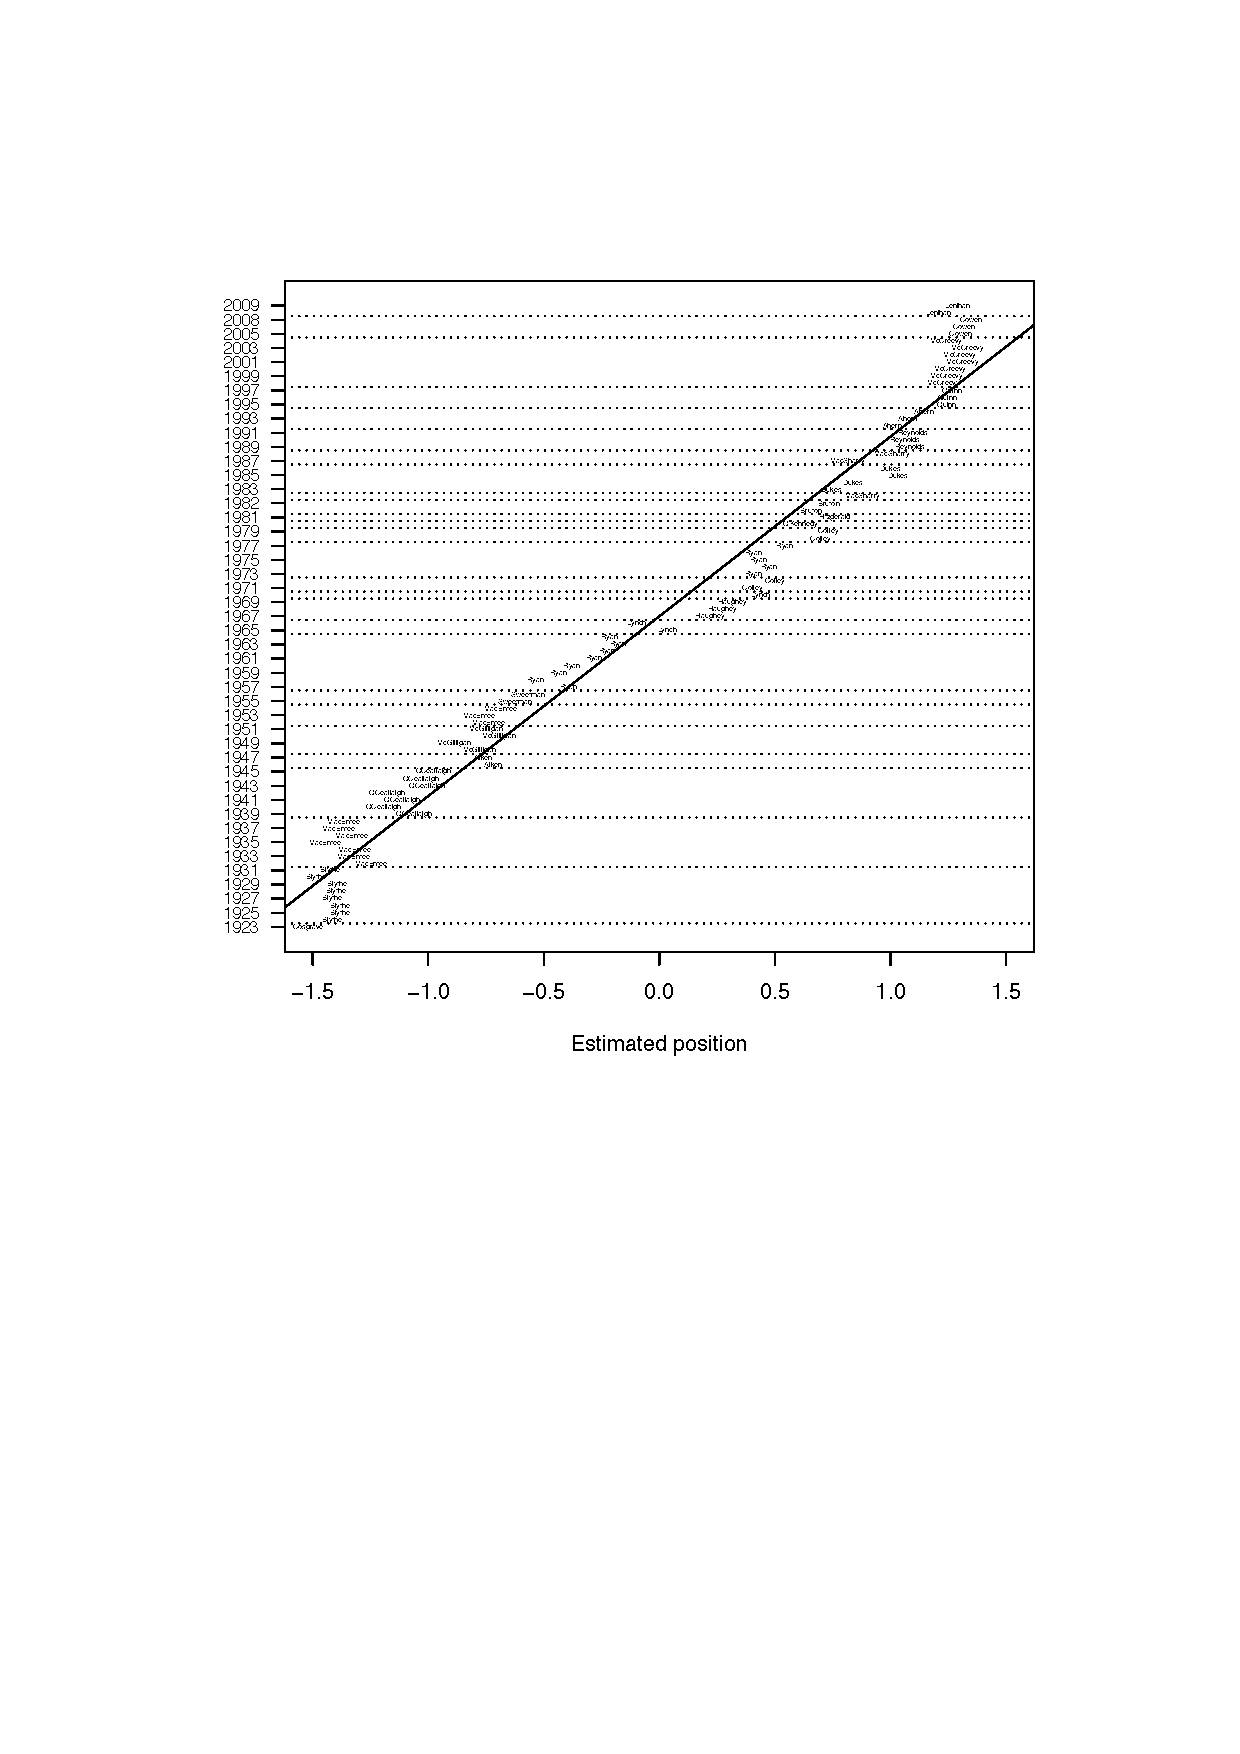
\includegraphics[scale=.9]{pictures/HandMfig2}}



\slide{Policy Dimensionality}

Emerging consensus: \vspace{0.2cm}

Identifying  policy dimensions in text is about vocabulary choice: substantive issue.

Different routes on how to get there are possible. 

Should be theory driven; validity is a big concern. 


\slide{A Note on Parliamentary Speeches}

Proksch and Slapin (2012):

\ita

\itm The "plenary bottleneck" of parliamentary politics: not all legislators will be able to speak in parliament on a given debate

\itm There may be strategic selection with regard to the speaker and the content of the speech

\itm Party leaders more involved in party-centered political systems, less in candidate-centered systems. This has consequences for the representation of preferences {\bf inside} a political party

\itm Important to understand the strategic context if you are interested in estimating individual MP positions 
\itz



\slide{Scaling in Context}

Scaling methods are indeed unobtrusive\ldots

But \textit{expressed positions} are almost always embedded in an institutional and strategic context
\ita
\itm Parliamentary speeches

\itm Even party platforms (the best case for selection issues) have variable audiences
\itz

~\\
and we're right back into models of politics\ldots 

\slide{}

\slide{Doing it at Home}

A `logit party position' data set is available from Ken Benoit

Wordfish and Wordscores are in the R package `austin'

Correspondence analysis is in the R package `MASS' (and many other places)

~\\
Doing at at someone else's home\ldots



\slide{}

\centerline{\includegraphics[scale=1]{pictures/dontputallyourheadsinonebasket}}


















\end{document}

%%%%%%%%%%%%%



%:ENDOFIMPORTED TOOLSFORTEXT



\slide{Of Left and Right}

Political representation is effective -- democratic, legitimate -- if politicians' preferences have the \textsl{right relationship} to citizens' preferences.

Spatial politics assumptions:
\ita
\itm 1) Policy preferences are \textit{positions} or \textit{ideal points} on policy \textit{dimensions}
\itm 2) There exists a \textit{low-dimensional space} that explains the multitude of positioning information available in observations of politics
\itz
Take everyday talk about `left' and `right' seriously.

\slide{Raw Materials of Left and Right}

Quantitative positioning information:
\ita
\itm Votes in a legislature (obvious, but biased)
\itm Answers to survey questions (unbiased but only sometimes possible)
\itm Structured qualitative analysis of manifestos (e.g. Pellican, Krouwel)
\itm Counts of policy promises or assertions in a manifesto or speech \citep[e.g.][]{Budgetal87}
\itm Frequencies of individual words \citep[e.g.]{Laveretal2003}
\itz

\slide{Of Left and Right}

\centerline{\includegraphics[scale=.7]{pictures/local-maastricht}}

Keiskompass (see also Wahl-o-mat).

\slide{Of Left and Right}

Two important issues:
\ita
\itm How to \textit{infer} positions (understanding, identifying, `scaling')
\itm How to \textit{take} positions (generation, `positioning')
\itz

These are connected practically, theoretically, and methodologically
%
%\slide{Of Left and Right}
%
%Theory:
%\ita
%\itm Position taking processes must be in `communicative equilibrium' with position inference processes
%\itz
%Methodology:
%\ita
%\itm Scaling methods for position inference should mirror generative assumptions about position taking
%\itm Statistically, this leads inevitably to a measurement model framework
%\itz
%
\slide{Measurement Models}

~\\
\centerline{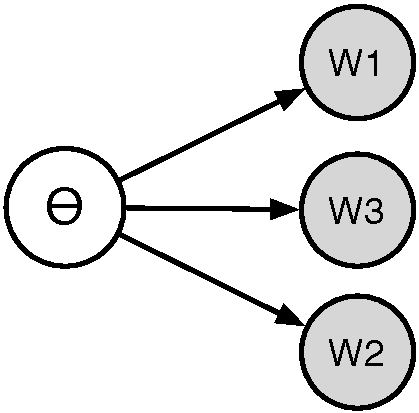
\includegraphics[scale=1]{pictures/gen}}

\slide{Measurement Models}

~\\
\centerline{\includegraphics[scale=1]{pictures/inf}}

%\slide{Words as Data}
%
%This approach to political text is part of the `words as data' movement in political science
%
%Focus: 
%\ita
%\itm \textit{How to do things with words} \citep{Austin1962,Searle1969}
%\itz
%Today: 
%\ita
%\itm Quantitative models of how to use words to take a position on an issue
%\itz
%Statistically we shall assume that positional information is \textit{signal} and everything else is \textit{noise} 
%


%
%\slide{Inferring Positions from Words}
%
%Previous work:
%\ita
%\itm Wordscores \citep{Laveretal2003}
%\itm Rhetorical Ideal Points \citep{MonroeMaeda04} 
%\itm Wordfish \citep{SlapinProksch2008}
%\itz
%
%\slide{Inferring Positions from Words}
%
%\centerline{\includegraphics[scale=.45]{wordscores-uk-ie}}
%
%\slide{Inferring Positions from Words}
%
%\centerline{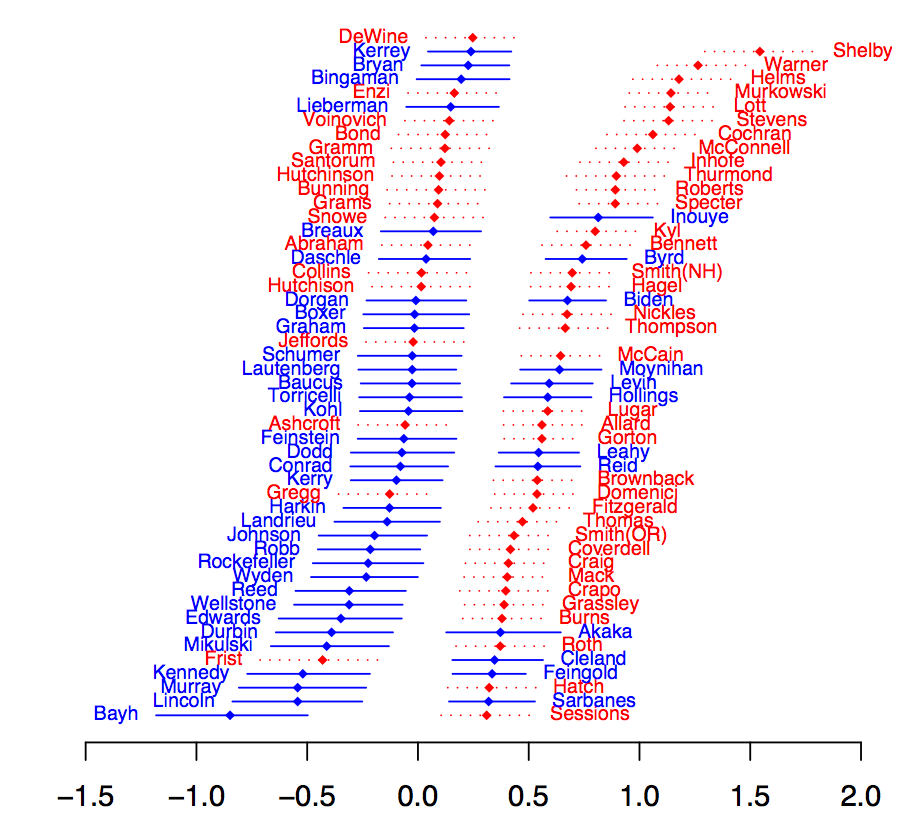
\includegraphics[scale=.45]{senator-ip-monroe-maeda}}
%
%\slide{Inferring Positions from Words}
%
%~\\
%\centerline{\includegraphics[scale=1.3]{clean-snap}}
%
%\slide{Inferring Positions from Words}
%
%Various approaches, motivations, and applications
%
%Also, \textit{unclear substantive assumptions, biases, methodological flaws} and \textit{downright mysteries}
%
%\ldots clarified by putting things in comparative perspective
%
%\slide{Position Inference}
%
%Educational Testing \citep[e.g.][]{BakerKim04}: 
%\ita
%\itm Item Response Theory models infer individual abilities (`positions') from test items (`words')
%\itz
%
%Psychology \citep[e.g][]{EmbretsonReise2000}
%\ita
%\itm Generalized Latent Trait models infer psychological traits (`positions') from, well, anything \citep{MoustakiKnott2000}
%\itz
%
%~\\
%Stolen Goods: A {focus} on the \textit{form} of $\theta \longrightarrow W$, the `item characteristic curve'
%
%\slide{Wordfish: $\theta \longrightarrow W_{j}$}
%
%~\\
%\includegraphics[scale=.7]{log-lambda.pdf}\hfill
%\includegraphics[scale=.7]{lambda.pdf}
%
%~\\
%The underlying Poisson regression model reflects a \textit{multiplicative} relationship between position and words used
%
%%\itm {sentence counts} (Budge 1994; Elff 2008) 
%
%\newpage
%
%\centerline{\includegraphics[scale=.75]{sp-informativeness.png}}
%
%\slide{Wordfish: $\theta \longrightarrow W_{j}$}
%
%What does Wordscores assumes about position making?
%
%We need to dip into the community ecology literature \citep[e.g.][]{terBraakPrentice2004}
%
%It's helpful to read the literature on\ldots
%
%\slide{Wolf Spiders}
%
%~\\
%\centerline{\includegraphics[scale=1]{125235799539}}
%
%\centerline{Nom, nom, nom}
%
%\slide{Wolf Spiders}
%
%\centerline{\includegraphics[scale=.6]{wolf-spiders}}
%
%Dune composition is `position'\\ 12 species of wolf spiders are `words'
%
%\slide{Wordscores: $\theta \longrightarrow W_{j}$}
%
%~\\
%\includegraphics[scale=.7]{log-wf}\hfill
%\includegraphics[scale=.7]{wf}
%
%Ignoring $\tau_{j}$ and $c_{j}$ leads to correspondence analysis
%
%\slide{Interdisciplinarity: Why Bother?}
%
%Insights from IRT and community ecology allow us to:
%
%Wordfish
%\ita
%\itm Estimate the model 20\% faster
%\itm Replace the inefficient bootstrap procedure for standard errors with an cheap equivalent (2 days versus 10 seconds)
%\itz
%Wordscores
%\ita
%\itm Diagnose bias and inefficiency
%\itm Extend the methods to infer postions on multiple dimensions
%\itz
%\citep{Lowe2008,LoweWF}
%
%\slide{Next Up: Psychophysics}

\slide{Positions from Coded Sentences}

What if we have policy categorizations for every sentence?
\ita
\itm e.g. Comparative Manifesto Project \citep{Budgetal87}
\itz
How to infer policy positions?

~\\
We'll consider two old methods of inferring a position from counts of sentences in one of 56 policy categories

And an substantial improvement\ldots

Then we'll get away from sentence coding and back to words, words, words\ldots

%
%\slide{CMP}
%
%  \scriptsize
%  \begin{tabular}{lll}
%    \toprule
%    {\bf Policy dimension}&{\bf ``Left'' Position}&{\bf ``Right''
%      Position}  \\ \midrule 
%Foreign alliances  & 101 Foreign Special Relationships: Positive &
%102: Foreign Special Relationships: Negative \\[1ex] 
%Militarism &  105 Military: Negative & 104 Military: Positive \\[1ex] 
%Internationalism & 107 Internationalism: Positive & 109
%Internationalism: Negative \\[1ex] 
%EU & 108 European Integration: Positive & 110 European Integration:
%Negative  \\[1ex] 
%~\\
%Traditional morality & 604
%Traditional Morality: Negative  & 603 Traditional Morality: Positive\\[1ex] 
%Multiculturalism & 607 Multiculturalism: Positive & 608
%Multiculturalism: Negative \\[1ex]
%Labour policy & 701 Labour Groups: Positive & 702 Labour Groups:
%Negative \\[1ex] 
%\bottomrule
%\end{tabular}
%\normalsize

\slide{Inferring Positions from Sentences}

Raw materials
\ita
\itm N sentences in a party manifesto
\itm L sentences coded into categories on one side of the issue
\itm R sentences coded into categories on the other side of the issue
\itz

\slide{How Not To Measure Position: CMP}

Intuition: The \textsl{difference} between right and left.

Comparative Manifesto Project position (from saliency theory)
\[
\theta^{(S)} ~=~ \frac{R-L}{N}
\]
Marginal effect: 1/N

Problems:
\ita
\item[-] Fixed (but hidden) end points
\item[-] Position depends on attention to \textit{other} issues  
\itz

\slide{How Not To Measure Position:\\Kim and Fording}

Intuition: The \textit{difference} between right and left \textsl{within the issue}

Relative position:
\[
\theta^{(R)} ~=~ \frac{R-L}{R+L}
\]
Marginal effect: 1/(R+L)

Problem:
\ita
\itm Fixed end points (that are often reached)
\itz

\citep{KimFording2002,LaverGarry2000}

\slide{How to Measure Position}

Intuition: The \textsl{balance} or \textit{relative emphasis} of R versus L

Empirical logit:
\[
\theta^{(L)} ~=~ \log\frac{R}{L} ~=~ \log(R) - \log(L)
\]

\textsl{No} fixed end points

Marginal effect: Depends on how much R or L there is already!

(Lowe et al. 2011)

\slide{How to Read a Text:\\ Marginal Effects}

A party manifesto from the most recent EP elections

\newpage

\footnotesize
Immigration is out of control.
\normalsize

\newpage

\footnotesize
Immigration is out of control.
\textbf{Britain's population is now over 60 million and rising, solely due to immigration.}
\normalsize

\newpage

\footnotesize
Immigration is out of control.
Britain's population is now over 60 million and rising, solely due to immigration.
\textbf{Not only is Britain increasingly overcrowded but the fact is that a country is the product of its people  and
if you change the people you will inevitably change the nature of the country.}
\normalsize

\newpage

\footnotesize
Immigration is out of control.
Britain's population is now over 60 million and rising, solely due to immigration.
Not only is Britain increasingly overcrowded but the fact is that a country is the product of its people  and
if you change the people you will inevitably change the nature of the country.
\textbf{We want Britain to remain - or return to - the way it has traditionally been.}
\normalsize

\newpage

\footnotesize
Immigration is out of control.
Britain's population is now over 60 million and rising, solely due to immigration.
Not only is Britain increasingly overcrowded but the fact is that a country is the product of its people  and
if you change the people you will inevitably change the nature of the country.
We want Britain to remain - or return to - the way it has traditionally been.
\textbf{We accept that Britain will always have ethnic minorities and 
have no problem with this as long as they remain minorities and
neither change nor seek to change the fundamental culture and identity of the indigenous peoples of the British Isles.}
\normalsize

\newpage

\footnotesize
Immigration is out of control.
Britain's population is now over 60 million and rising, solely due to immigration.
Not only is Britain increasingly overcrowded but the fact is that a country is the product of its people  and
if you change the people you will inevitably change the nature of the country.
We want Britain to remain - or return to - the way it has traditionally been.
We accept that Britain will always have ethnic minorities and 
have no problem with this as long as they remain minorities and
neither change nor seek to change the fundamental culture and identity of the indigenous peoples of the British Isles.\\
~\\
\textbf{The current open-door policy and unrestricted uncontrolled immigration is leading to higher crime rates, demand for more housing (driving prices out of the reach of young people), severe strain on the environment, traffic congestion, longer hospital waiting list, lower educational standards, higher income taxes, lower wages, higher unemployment, loss of British identity, a breakdown in community spirit, more restrictive policing, higher council tax rates, a shortage of council homes, higher levels of stress and unhappiness and a more atomized society.}
\normalsize

\slide{The Psychophysics of\\ Left and Right}

Inferences about position operate like perceptions of loudness or perceived weight 

The smallest perceivable \textsl{policy position} difference (JND) depends on the extremity of the existing policy.

\ita
\itm This is the Weber-Fechner Law \citep{Fechner1965}
\itz

\slide{The Psychophysics of\\ Left and Right}

For log ratio scales: 
\ita
\itm Assume $\theta^{(L)}=0$ with N=10
\itm Add \textit{one more R} sentence: $\theta^{(L)}\approx 0.4$
\itm Assume $\theta^{(L)}=0$ with N=50
\itm Add \textit{one more R} sentence: $\theta^{(L)}\approx 0.08$
\itz


\slide{The Psychophysics of\\ Left and Right}

~\\
Compare these possible measures to expert survey scores \citep{BenoitLaver2006}

\newpage

\begin{center}
    \includegraphics[scale=0.8]{pictures/proofSocial.pdf}
\end{center}
\newpage

\begin{center}
   \includegraphics[scale=0.8]{pictures/proofMulticult.pdf}
\end{center}
\newpage

\begin{center}
    \includegraphics[scale=0.8]{pictures/proofEnvt.pdf}
\end{center}

\slide{Just a Moment\ldots}

Did you say environmental policy positions?  Surely nobody says anything \textit{against} the environment

\slide{Just a Moment\ldots}

True.  They choose something else to emphasize instead\ldots

~\\
The Danish Liberal Party in 1988:

\ita
\itm ``Milj\o politikken m\aa ikke stille danske virksomheder d\aa rligere, end
  virksomhederne i de lande vi konkurrerer med''
\itm Environmental policy should not result in Danish companies
  being worse off than the companies in the countries with which we
  compete.
\itz

\slide{Look Ma, No Model}

This is not a  \textsl{model} of $\theta$, its dimensionality, determinants, or structure.  Just a way to figure out what it is from text.

This is a \textsl{noisy} scaling technique compared to, e.g. indexes from carefully focused survey questions or expert opinion.  A model would help here\ldots

The \textsl{form} of decreasing marginal effects -- here the log -- is assumed, and supported by comparison to expert scores, but needs empirical confirmation \citep{Stevens1957}

\slide{Other Possibilities}

\centerline{\includegraphics[scale=.6]{pictures/stevens.png}}

Stimulus intensity = more L (or R) words.\\
Sensation magnitude = position movement left (or right)

\slide{Some Testable Empirical Consequences}

Opportunity cost effects:
\ita
\itm Larger $L+R$ allows more \textit{precision} about inferred position (e.g. UK 1997 New Labour manifesto)
\itm possibly at the expense of precision about position on \textsl{other} issues
\itm Decreasing marginal effects and fixed word budgets force parties with extreme positions to be single issue 
\itz

Preferences inferred from compositional data (like coded text) will not, in general, be Euclidean \citep{Milyo2000}.

\slide{What if we have only words?}

The basic \textit{data} is the frequency matrix $W$
\ita
\itm $N$ Documents $\times$ $V$ Words 
\ita
\itm (speeches and words, parties and words, speakers and words, etc.)
\itz
\itm $W_{ij}$ is the number of times $j$ appears in $i$
\itz

~\\
Underneath the numbers each actor has a position $\theta_{i}$ on a latent dimension

That position explains why individual word occurrences are correlated

\slide{Approaches that Won't Work}

Go for $\theta \Longleftarrow W$ directly

~\\
\textit{Linear regression} of $\theta$ on $W$
\ita
\itm $\theta$ is not directly observed
\itm Even if it were, the model would over-fit horribly
\itz

\textit{Classification} of $\theta$ using $W$
\ita
\itm Requires $\theta$ to be redefined as categorical
\itm $\theta$ is still not observed
\itz

\slide{Approaches that Will Work}

Get $\theta$ from W {indirectly} by modeling $W \longleftarrow \theta$ and reversing it

~\\
Latent variable models
\ita
\itm Factor Analysis, Item Response Theory and Latent Trait Models
\itm Unfolding, Multidimensional Scaling  
\itz



\slide{ Assumptions}

Assume
\ita
\itm Positions are unidimensional in $W$ 
\itm Positions drive word counts stochastically according to $P(W_{j} \mid \theta)$
\itm Counts of $W_{j}$ are conditionally independent given $\theta$
\[
P(W_{1}\ldots W_{V}) ~=~ \prod^{V}_{j} P(W_{j} \mid \theta)~ P(\theta)
\] 
\itz 

\slide{Models}

We focus on:
\ita
\itm \textit{Wordscores} (Laver et al. 2003)
\itm \textit{Wordfish}: (Slapin and Proksch, 2008)
\itm (Also Monroe and Maeda, 2004; Beauchamp, 2008; Pennings and Keman, 2002; K\"{o}nig and Luig, 2009)
\itz


~\\
Wordscores and Wordfish make different assumptions about $P(W_{j} \mid \theta)$ and about how to deal with dimensions


\slide{Wordfish}

The position word relationship is
\begin{eqnarray*}
W_{ij} &\sim& \text{Poisson}(\mu_{ij})\\
\log \mu_{ij} &=& \psi_{j} + \beta_{j}\theta_{i} +  \alpha_{i} 
\end{eqnarray*}
Each word is a Poisson Process driven by word and document parameters

Word parameters:
\ita
\itm $\beta$~~ how fast counts increase or decrease with changes in position
\itm $\psi$~~ how frequent words are irrespective of position
\itz

\slide{Wordfish}

~\\
~\\
\centerline{\includegraphics[scale=.75]{pictures/log-lambda}\quad\quad\quad\includegraphics[scale=.75]{pictures/lambda}}

\slide{Wordfish}


Ideal data:
\footnotesize
\begin{verbatim}
    D1 D2 D3 D4 D5 D6 D7 D8 D9 D10
W1   6 12  5 13 30 19 38 43 44  47
W2   2  4  9  7 29 21 40 33 43  43
W3   6  3  2  6 20 27 28 42 47  49
W4   4  7  7  9 34 27 30 38 47  48
W5   2  6  7 13 25 36 24 31 32  52
...
W11 50 46 49 38 21 27 17  7  5   1
W12 53 39 46 35 20 26 18 10 12   4
W13 36 51 39 46 27 18 19  8  3   2
W14 46 46 43 43 24 20 13  7 10   1
W15 43 44 35 35 25 30 15  8 12   3
\end{verbatim}
\normalsize



\newpage

\slide{Wordfish}
\centerline{\includegraphics[scale=.5]{pictures/sp-informativeness}}


\slide{Wordfish}

The position word relationship is
\begin{eqnarray*}
W_{ij} &\sim& \text{Poisson}(\mu_{ij})\\
\log \mu_{ij} &=& \psi_{j} + \beta_{j}\theta_{i} +  \alpha_{i}
\end{eqnarray*}
Each word is a Poisson Process driven by word and document parameters

Document parameters:
\ita
\itm $\theta$~~ the position being expressed
\itm $\alpha$~~ the umm\ldots well, it's kind of\ldots
\itz

\slide{Wordfish}

If document \textit{length} is uninformative about position then we can condition on it

If Wordfish's heroic assumptions are true then conditioning on document length gives an alternative form of the model
\begin{eqnarray*}
P(W_{i} \mid \theta_{i}, N) &=& \text{Multinomial}(\boldsymbol{\pi}, N)\\
\log \frac{\pi_{ij}}{\pi_{i1}} &=& \psi^{*}_{j} + \beta^{*}_{j}\theta_{i}
\end{eqnarray*}
where $\psi^{*}_{j} \leftarrow (\psi_{j}-\psi_{1})$, $\beta^{*}_{j} \leftarrow (\beta_{j}-\beta_{1})$ and $\alpha_{i}$ cancels

~\\
Wordfish is secretly a Multinomial Response Model ($\alpha$ recovers the document length margin)


\slide{Estimation}

Wordfish models are fit using Conditional Maximum Likelihood
\ita
\itm (Not \textit{quite} an EM algorithm, but works in practice)
\itz

Iterate:
\ita
\itm Fix $\alpha$ and $\theta$ and maximize $\beta$ and $\psi$
\itm Fix $\beta$ and $\psi$ and maximize $\alpha$ and $\theta$
\itz

This can be quite slow\ldots

The model is slightly more stable when $\beta$ is regularized 
\ita
\itm Equivalent to assuming that $\beta \sim \text{Normal}(0,\sigma^{2})$ a priori
\itz

\slide{A Hint of Bayes}

The iteration embeds an application of Bayes theorem:
\ita
\itm In step 2: Assume $P(\theta)$ is constant
\begin{eqnarray*}
P(\theta \mid W; \beta, \psi) &~\propto~& P(W \mid \theta; \beta, \psi)~ P(\theta)\\
\text{Posterior} &~\propto~& \text{Likelihood} ~\times~ \text{Prior}\\
\theta \Longleftarrow W & & W \longleftarrow \theta,\quad \theta
\end{eqnarray*}
Maximize this posterior distribution over $\theta$
\itz
~\\
Note that the Likelihood is really $V$ Likelihoods, one for each word type\ldots

\slide{Recap: The Likelihood}

For any statistical model -- Regression, Wordfish, Factor analysis -- there are two components:
\ita
\itm The model assumptions, e.g. linearity and Poisson observations
\itm The parameters in that model, $\theta$, $\beta$, etc.
\itz
Different parameter values make an entire data set more or less likely, e.g. we define a \textit{likelihood} of the data.

This is a function of all the parameters that has a \textit{peak} at the values that make the data \textit{most probable}

The basic estimation issue is: how do we get to that peak?


\slide{(Not Much) Uncertainty}

\centerline{\includegraphics[scale=.85]{pictures/poissonscaling}}

\slide{(Not Much) Uncertainty}

If word counts \textit{are} conditionally independent given $\theta$ then (depending on $\beta$) each word gives a new bit of information about position

They probably aren't.  So it probably doesn't.

~\\
Word counts may be over-dispersed relative to the Poisson assumption because
\ita
\itm Non-positional information -- rhetoric, explanation, grammar -- might not just be noise
\itm Other dimensions may be lurking in $W$ 
\itz

But it's a start\ldots



\slide{Wordscores}

Wordscores was presented as an \textit{algorithm} not a \textit{model}, but we can figure out
\ita
\itm Each word $j$ has a policy position or `word score' $\pi_{j}$
\itm Some `reference' document positions are \textit{known}.
\itm Symmetry:
\ita
\itm Document positions are the average of their words' positions
\itm So word positions are the average position of documents they appear in
\itz
\itz
Algorithm:
\ita
\itm 1. Compute $\pi$ as the frequency weighted average of document scores
\itm 2. Compute new $\theta$ as the frequency weighted average of wordscores
\itz


\newpage

\centerline{\includegraphics[scale=.5]{pictures/wordscores-uk-ie.png}}


\slide{Wordscores}

Estimate the probability of seeing a word \textsl{given} that we are reading a particular document

Use W
\begin{align*}
{P}(w_j \mid d_i) &= \frac{c(\text{word j in i})}{c(\text{all words in i})} ~~=~~ \frac{{W}_{ij}}{\sum_j {W}_{ij}}
\end{align*}
If we just see $w_j$, what is the probability we are in document 1?  document 2?

\slide{Estimating Probabilities}

Use the word frequency matrix:
\begin{verbatim}
         farm, farmer, farmers, farming 
uklab92,     1      0        1        2
uklab97,     0      0        0        0
uklab01,     1      0        2        7   
uklab05,     0      1        1        0
...
\end{verbatim}
If these were the only words in the manifesto
\begin{align*}
P(W=\text{'farm'} \mid d=\text{'uklab01'}) ~=~ 1/10 ~=~ 0.1
\end{align*}

\slide{Wordscores}

Use this information to compute the probability of being in \texttt{uklab01} given we see the word \texttt{farming} once

Bayes theorem (again assuming $P(d_i)$ is constant)
\begin{align*}
P(d_i \mid w_j) &~=~ \frac{P(w_j \mid d_i)~P(d_i)}{\sum_j P(w_j \mid d_i)~P(d_i)} ~~=~~\frac{P(w_j \mid d_i)}{\sum_i P(w_j \mid d_i)}
\end{align*}

Symmetry:
\ita
\itm So we have $P(d_i \mid w_j)$ and $P(w_{j} \mid d_i)$
\itz

\slide{Wordscores}

Symmetrical estimation strategy:
\begin{align*}
\pi_{j} &~=~  \sum^{R}_{i} \theta_{d_{i}} P(d_i \mid w_j)\\
\theta_{i} &~=~ \sum^{V}_{j} \pi_{w_{j}} P(w_{j}\mid d_i)\\
\end{align*}


All very nice\ldots but what are we assuming when we do this?

\slide{Wordscores: Reconstruction}

~\\
\centerline{\includegraphics[scale=.75]{pictures/log-ws}\quad\quad\quad\includegraphics[scale=.75]{pictures/ws}}

~\\
Assume $\tau_{j}$ and $c_{j}$ are the \textit{same} for all words: We get Correspondence Analysis

Assume some $\theta$ are known: We get Wordscores

\newpage
\centerline{\includegraphics[scale=.65]{pictures/apsrtable}}

\slide{Estimation}

Iterate:
\ita
\itm Fix $\theta$ and compute $\pi$
\itm Fix $\pi$ and compute $\theta$
\itz

Wordscores models are fit by doing this once

\textit{Continuing} the steps (and treating all texts as in-sample) leads to a correspondence analysis
\ita
\itm In Austin: Classic Wordscores vs. Wordscores
\itz
This is super fast\ldots

(The iteration embeds an application of Bayes theorem, kinda)

\slide{(Lack of) Uncertainty}

Laver et al. offer standard errors for Wordscores analysis

Be wary of these:
\ita
\itm Correspondence Analysis provides no generative probability model
\itm Errors \textit{shrink} as documents take more extreme positions
\itz

Bootstrapped standard errors are possible, but their theoretical properties need to be worked out

\slide{Compare and Contrast}

Wordfish estimates of $\theta$ \textsl{control} for 
\ita
\itm different word frequencies ($\psi$) 
\itm different levels of ideological relevance of words ($\beta$). 
\itz
Words do not have an ideological position themselves, only a sensitivity to the \textit{speaker's} ideological position

~\\
For `short' dimensions the two stories about $P(W\mid\theta)$ can look pretty similar. 

%\slide{Big Picture: As Measurement}
%
%\begin{center}
%\footnotesize
%\begin{tabular}{ccc}
%\textbf{Distance Measures} & \textbf{Dominance Measures} & \\
% &  & \\
%Parametric Unfolding & Item Response Theory & (Wordfish) \\ 
%$\uparrow$ & $\uparrow$ & \\
%\textsl{approx.} & \textsl{approx.} & \\
%$\mid$ & $\mid$ & \\
%Correspondence Analysis & Factor Analysis & \\
%$\uparrow$ & $\uparrow$ & \\
%\textsl{implements} & \textsl{approx.} & \\
%$\mid$ & $\mid$ & \\
%Reciprocal Averaging & PCA & \\
%$\uparrow$ & & \\
%\textsl{approx.} &  & \\
%$\mid$ & & \\
%Wordscores & & \\
%\end{tabular}
%\normalsize
%\end{center}


\slide{Dimension Issues}

What the heck is $\theta$?

How do we know that positions on only one dimension are being expressed in the text?

\slide{Dimension Issues}

What the heck is $\theta$?
\ita
\itm Whatever maximizes the Likelihood
\itm Approximately the first principal component of $\log W$ 
\itz
Wordfish is effectively \textit{exploratory} -- you have to figure out what the dimension really is

\slide{Dimension Issues}

\centerline{\includegraphics[scale=1]{pictures/ep}}

Proksch and Slapin, 2009

NOMINATE 2 was the best predictor, but not necessarily a particularly good one\ldots

\slide{Worst Case Scenario}

\centerline{\includegraphics[scale=1]{pictures/HandMfig2}}



\slide{Dimensional Issues}

For Classic Wordscores, Laver et al. claim that choice of reference documents determines the identity of $\theta$ and restricts positional information to that dimension
\ita
\itm With exactly 2 reference texts this \textit{cannot be true}.
\ita
\itm 2 texts only identify scale and direction
\itz
\itm With more than 2 reference texts the claim is intriguing, but unproven
\itz
For Correspondence Analysis, there are no reference texts but more than one dimension can be extracted

That dimension is simply \textit{orthogonal} to the previous ones.

\newpage
\centerline{\includegraphics[scale=.65]{pictures/apsrtable}}

\slide{Identifying Dimensionality: The Arch}

\centerline{\includegraphics[scale=.75]{pictures/ca2}}

\slide{Emerging Consensus about Dimensionality}

Identifying and isolating the policy dimension is about \textit{vocabulary choice}
\ita
\itm Scale with only `defense' words: get a defense dimension
\itm Scale with all words: get a \textit{salience-weighted average} dimension
\itz

Chopping up the text into single topic sections effectively focuses on the vocabulary particular to that topic.

Fitting multiple dimensions and rotating to simple structure does the same

If setting reference scores also focus the vocabulary, that would justify them\ldots

\slide{Mixing Topics}

Scaling speeches from the most recent Irish budget debate:

~\\
\centerline{\includegraphics[scale=1.2]{pictures/mixed-snap}}

\slide{Who is John Gormley?}

\centerline{\includegraphics[scale=1.3]{pictures/gormley-the-man-himself}}

John Gormley: leader of the Green Party \textit{and} Minister for the Environment, Heritage and Local Government

\slide{Who is John Gormley?}

``As leader of the Green Party I want to take this opportunity to set out my party's position on budget 2010 \ldots ''

[772 words later]

``I will now comment on some specific aspects of my Department's Estimate. I will concentrate on the principal sectors within the Department's very broad remit \ldots ''

\slide{Unmixing Topics}

Ministerial text removed:

~\\
\centerline{\includegraphics[scale=1.2]{pictures/clean-snap}}

\slide{More Dimensional Issues}

Two dimensions:
\ita
\itm government and opposition
\itm economic left-right
\itz

In Correspondence Analysis: 
\ita
\itm Removing the data for Gormley's ministerial positioning leaves his left-right positions
\itz

In Classic Wordscores: 
\ita
\itm Cowen and Kenny's speeches define the word scores, which seem to reflect left-right more than government and opposition
\itz

\slide{Selection Bias}

All scaling models assume sampling that is 
\ita
\itm simple random, or 
\itm conditioned on factors unrelated to position
\itz

Positions scaled from roll-call votes may be biased, e.g. if non-contentious issues disproportionally get voted on (Carrubba et al.)

Positions from text may be biased depending on the selection process
\ita
\itm e.g. legislative speech: 
\ita
\itm Party control of speaking opportunities, chamber speaking rules, responsive debate speech
\itz
\itz

\slide{Scaling in Context}

Scaling methods are indeed unobtrusive\ldots

But \textit{expressed positions} are almost always embedded in an institutional and strategic context
\ita
\itm Even party platforms (the best case for selection issues) have variable audiences
\itz

~\\
and bang -- we're right back into models of politics\ldots


\slide{}




%
%\slide{Only Connect}
%
%The exponentially increasing ICC for Wordfish models of \textit{words}, and the empirical logit function for relative emphasis of \textit{sentences} are {deeply connected}
%\ita
%\itm (Wordfish actually has a useful parameterization in logits)
%\itz
%
%Both treat position taking as multiplicative rather than additive
%
%Unification: 
%\ita
%\itm All effective scaling models make essentially the same assumptions\ldots
%\itm `Perception' of left and right is just like\ldots perception 
%\itz
%\slide{S\"{u}\ss igkeiten}
%
%A \textsl{data set} of party positions on 5 old, 11 specific, and 3 totally new scales
%\ita
%\item[-] Left-right, planned v. market economy, welfare and social security, pro-/anti-EU, social liberalism
%\item[-] Foreign alliances,	militarism , internationalism, constitionalism, decentralisation, protectionism, Keynesian policy, nationalism, traditional morality, multiculturalism, labour policy
%\item[-] Environmental protection v. growth economy, free-market economy, state provision of social services.
%\itz
%
%\slide{S\"{u}\ss igkeiten}
%
%\begin{center}
%\textbf{Austin}
%
%\includegraphics[scale=2]{austin-beta}\\
%
%An R package for doing things with words
%\end{center}
%

\bibliographystyle{apsr}
\bibliography{all}

\end{document}

%%%%%%%%%%%%%%%%%%%%%%%%%%%%%%%%%%%%%%%%%%%%%%%%%%%%%%%%%%


%
%
%\slide{What You Get Today}
%
%A new \textsl{method} for inferring continuous policy positions from coded text
%
%
%A \textsl{demonstration} that it is better than existing methods
%
%A \textsl{data set} of party positions on 5 old, 11 specific, and 3 totally new scales
%\ita
%\item[-] Left-right, planned v. market economy, welfare and social security, pro-/anti-EU, social liberalism
%\item[-] Foreign alliances,	militarism , internationalism, constitionalism, decentralisation, protectionism, Keynesian policy, nationalism, traditional morality, multiculturalism, labour policy
%\item[-] Environmental protection v. growth economy, free-market economy, state provision of social services.
%\itz
%
%
%
%
%
%\slide{The Ingredients of Position}
%
%We have as raw materials:
%\ita
%\itm N sentences in a party manifesto
%\itm L sentences coded into categories on one side of the issue
%\itm R sentences coded into categories on the other side of the issue
%\itz
%
%For any \textsl{measure} we can ask:
%\ita
%\itm What is the \textsl{marginal effect} of another sentence in L (or R)
%\itm What is the effect of the position on \textsl{different} issues
%\itz


\slide{Approaches that Won't Work}

Go for $\theta \longleftarrow W$ directly

~\\
\textit{Linear regression} of $\theta$ on $W$
\ita
\itm $\theta$ is not directly observed
\itm Even if it were, the model would over-fit horribly
\itz

\textit{Classification} of $\theta$ using $W$
\ita
\itm Requires $\theta$ to be redefined as categorical
\itm $\theta$ is still not observed
\itz



\slide{(Not Much) Uncertainty}

If word counts \textit{are} conditionally independent given $\theta$ then (depending on $\beta$) each word gives a new bit of information about position

They probably aren't.  So it probably doesn't.

~\\
Word counts may be over-dispersed relative to the Poisson assumption because
\ita
\itm Non-positional information -- rhetoric, explanation, grammar -- might not just be noise
\itm Other dimensions may be lurking in $W$ 
\itz

But it's a start\ldots


\slide{Wordscores}

Wordscores was presented as an \textit{algorithm} not a \textit{model}, but we can figure out
\ita
\itm Each word $j$ has a policy position or `word score' $\pi_{j}$
\itm Some `reference' document positions are \textit{known}.
\itm Symmetry:
\ita
\itm Document positions are the average of their words' positions
\itm So word positions are the average position of documents they appear in
\itz
\itz

\slide{Wordscores}

Algorithm:
\ita
\itm 1. Compute $\pi$ as the frequency weighted average of document scores
\itm 2. Compute new $\theta$ as the frequency weighted average of wordscores
\itz

A word of advice:
\ita
\itm Distrust algorithms
\itz
(algorithms belong in appendices and replication materials)


\slide{Wordscores}
\centerline{\includegraphics[scale=.4]{pictures/wordscores-uk-ie.png}}


%\slide{Wordscores}
%
%Estimate the probability of seeing a word \textsl{given} that we are reading a particular document
%
%Use W
%\begin{align*}
%{P}(w_j \mid d_i) &= \frac{c(\text{word j in i})}{c(\text{all words in i})} ~~=~~ \frac{{W}_{ij}}{\sum_j {W}_{ij}}
%\end{align*}
%If we just see $w_j$, what is the probability we are in document 1?  document 2?
%
%\slide{Estimating Probabilities}
%
%Use the word frequency matrix:
%\begin{verbatim}
%         farm, farmer, farmers, farming 
%uklab92,     1      0        1        2
%uklab97,     0      0        0        0
%uklab01,     1      0        2        7   
%uklab05,     0      1        1        0
%...
%\end{verbatim}
%If these were the only words in the manifesto
%\begin{align*}
%P(W=\text{'farm'} \mid d=\text{'uklab01'}) ~=~ 1/10 ~=~ 0.1
%\end{align*}
%
%\slide{Wordscores}
%
%Use this information to compute the probability of being in \texttt{uklab01} given we see the word \texttt{farming} once
%
%Bayes theorem (again assuming $P(d_i)$ is constant)
%\begin{align*}
%P(d_i \mid w_j) &~=~ \frac{P(w_j \mid d_i)~P(d_i)}{\sum_j P(w_j \mid d_i)~P(d_i)} ~~=~~\frac{P(w_j \mid d_i)}{\sum_i P(w_j \mid d_i)}
%\end{align*}
%
%Symmetry:
%\ita
%\itm So we have $P(d_i \mid w_j)$ and $P(w_{j} \mid d_i)$
%\itz
%
%\slide{Wordscores}
%
%Symmetrical estimation strategy:
%\begin{align*}
%\pi_{j} &~=~  \sum^{R}_{i} \theta_{d_{i}} P(d_i \mid w_j)\\
%\theta_{i} &~=~ \sum^{V}_{j} \pi_{w_{j}} P(w_{j}\mid d_i)\\
%\end{align*}
%
%
%All very nice\ldots but what are we assuming when we do this?

\slide{Wordscores: Reconstruction}

~\\
\centerline{\includegraphics[scale=.75]{log-ws}\quad\quad\quad\includegraphics[scale=.75]{ws}}

~\\
Assume $\tau_{j}$ and $c_{j}$ are the \textit{same} for all words: We get Correspondence Analysis

Assume some $\theta$ are known: We get Wordscores

\newpage
\centerline{\includegraphics[scale=.65]{apsrtable}}

\slide{Estimation}

Iterate:
\ita
\itm Fix $\theta$ and compute $\pi$
\itm Fix $\pi$ and compute $\theta$
\itz

Wordscores models are fit by doing this once

\textit{Continuing} the steps (and treating all texts as in-sample) leads to a correspondence analysis

This is super fast\ldots

\slide{(Lack of) Uncertainty}

Laver et al. offer standard errors for Wordscores analysis

Be wary of these:
\ita
\itm Correspondence Analysis provides no generative probability model
\itm Errors \textit{shrink} as documents take more extreme positions
\itz

Bootstrapped standard errors are possible, but their theoretical properties need to be worked out

\slide{Compare and Contrast}

Wordfish estimates of $\theta$ \textsl{control} for 
\ita
\itm different word frequencies ($\psi$) 
\itm different levels of ideological relevance of words ($\beta$). 
\itz
Words do not have an ideological position themselves, only a sensitivity to the \textit{speaker's} ideological position

~\\
For `short' dimensions the two stories about $P(W\mid\theta)$ can look pretty similar. 

Empirically, position estimates tend to be similar





\slide{Dimension Issues}

\centerline{\includegraphics[scale=1]{ep}}

Proksch and Slapin, 2009

NOMINATE 2 was the best predictor, but not necessarily a particularly good one\ldots

\slide{Worst Case Scenario}

\centerline{\includegraphics[scale=1]{HandMfig2}}


\slide{Dimensional Issues}

How do we know that positions on only one dimension are being expressed in the text?

\textit{Make it so}
\ita
\itm Chop the text into sections that are guaranteed to be on the same topic and scale them separately
\ita
\itm Monroe and Quinn (endlessly forthcoming) use a topic model
\itm Slapin and Proksch do it manually
\itz
\itz
Advantages:
\ita
\itm Heroic assumptions are (closer to being) true
\itm No need to worry about interpretation (Workhorse/Showhorse?)
\itz

\slide{Dimensional Issues}

For Classic Wordscores, Laver et al. claim that choice of reference documents determines the identity of $\theta$ and restricts positional information to that dimension
\ita
\itm With exactly 2 reference texts this \textit{cannot be true}.
\ita
\itm 2 texts only identify scale and direction
\itz
\itm With more than 2 reference texts the claim is intriguing, but unproven
\itz
For Correspondence Analysis, there are no reference texts but more than one dimension can be extracted

That dimension is simply \textit{orthogonal} to the previous ones.

\newpage
\centerline{\includegraphics[scale=.65]{apsrtable}}

\slide{Identifying Dimensionality: The Arch}

\centerline{\includegraphics[scale=.75]{ca2}}

\slide{Emerging Consensus about Dimensionality}

Identifying and isolating the policy dimension is about \textit{vocabulary choice}
\ita
\itm Scale with only `defense' words: get a defense dimension
\itm Scale with all words: get a \textit{salience-weighted average} dimension
\itz

Chopping up the text into single topic sections effectively focuses on the vocabulary particular to that topic.

Fitting multiple dimensions and rotating to simple structure does the same

%If setting reference scores also focus the vocabulary, that would justify them\ldots




\slide{More Dimensional Issues}

Two dimensions:
\ita
\itm government and opposition
\itm economic left-right
\itz

In Correspondence Analysis: 
\ita
\itm Removing the data for Gormley's ministerial positioning leaves his left-right positions
\itz

In Classic Wordscores: 
\ita
\itm Cowen and Kenny's speeches define the word scores, which seem to reflect left-right more than government and opposition
\itz

\slide{Selection Bias}

All scaling models assume sampling that is 
\ita
\itm simple random, or 
\itm conditioned on factors unrelated to position
\itz

Positions scaled from roll-call votes may be biased, e.g. if non-contentious issues disproportionally get voted on (Carrubba et al.)

Positions from text may be biased depending on the selection process
\ita
\itm e.g. legislative speech: 
\ita
\itm Party control of speaking opportunities, chamber speaking rules, responsive debate speech
\itz
\itz

